\documentclass{article}
\usepackage{graphicx} % Required for inserting images
\usepackage{hyperref}
\usepackage{tikz}

\title{Project equivalent to written exam}
\author{
  Drago\c{s}-Alexandru Efrim\\
  Olivia Drobot
}
\date{May 2023}

\begin{document}

\maketitle

\section{Problem statement}
Starting from a database that is already in NF3, create a program that allows the user to perform CRUD (Create, Read, Update, and Delete) operations on the database. For this exercise, JPA annotations can be used, and to connect the database to IntelliJ, PostgreSQL will be used. Finally, write the steps for running the application for anyone who would like to test the project.

\section{Documentation}
\subsection{Links}
\begin{itemize}
    \item \href{https://www.jetbrains.com/idea/guide/tutorials/your-first-spring-application/creating-spring-boot-application/}{JetBrains - Used to create the application}
    \item \href{https://www.geeksforgeeks.org/spring-boot-application-properties/}{GeeksForGeeks - Used to connect to the PostgreSQL database}
    \item \href{https://www.bezkoder.com/spring-boot-postgresql-example/}{BezKoder - Used to create models, repositories, and controllers}
\end{itemize}

\section{Main programming tools used}
\begin{itemize}
    \item We configured the Spring Boot project to set the dependencies and have access to Jakarta Persistence, as well as other utilities, such as:
    \begin{itemize}
        \item @CrossOrigin - allows cross-origin resource sharing (CORS), enabling requests from a different domain to access the API endpoints in the controller
        \item @RestController - marks the class as a RESTful controller; it combines the @Controller and @ResponseBody annotations, indicating that the class will handle HTTP requests and return the response directly as the body of the response
        \item @RequestMapping - specifies the base URL mapping for all the endpoints in the controller
        \item @Autowired - used for automatic dependency injection in Spring
        \item @GetMapping - maps the HTTP GET request to the specified endpoint; it handles the retrieval of all objects from the database
        \item @PostMapping - maps the HTTP POST request to the specified endpoint; it handles the creation of a new object in the database
        \item @PutMapping - maps the HTTP PUT request to the specified endpoint; it handles the updating of a specific object identified by it's ID path variable
        \item @DeleteMapping - maps the HTTP DELETE request to the specified endpoint; it handles the deletion of all objects (or a specific one) from the database
        \item @RequestParam - is used in the method to specify a query parameter that is optional; it allows filtering based on the provided parameter
    \end{itemize}
    \item We have used Jakarta Persistence API (JPA) for storing, accessing and administrating data between the objects from Java and the PostgreSQL database
    \begin{itemize}
        \item @Entity - used to mark the class as an entity, representing a persistent object that is mapped to a database table; it indicates that instances of this class can be stored and retrieved from the database
        \item @Table - specifies the name of the database table to which the entity is mapped
        \item @Id - used to mark the field as the primary key of the entity; indicates that this field uniquely identifies each object
        \item @GeneratedValue - specifies the strategy for generating the values of the primary key
        \item @Column - maps the specific field to its corresponding column in the database table; it specifies the name of the column to which this attribute is persisted
    \end{itemize}
\end{itemize}
For organizing the project we have used multiple models, repositories and controllers:
\begin{itemize}
    \item Models - contains the classes that represent the data models of the application; these are Java objects that are mapped to database tables
    \item Repositories - contains the interfaces that handle data access and manipulation in the database
    \item Controllers - contains the classes that define the entry points of the application and handle the HTTP requests received from the client
\end{itemize}

\section{EER}
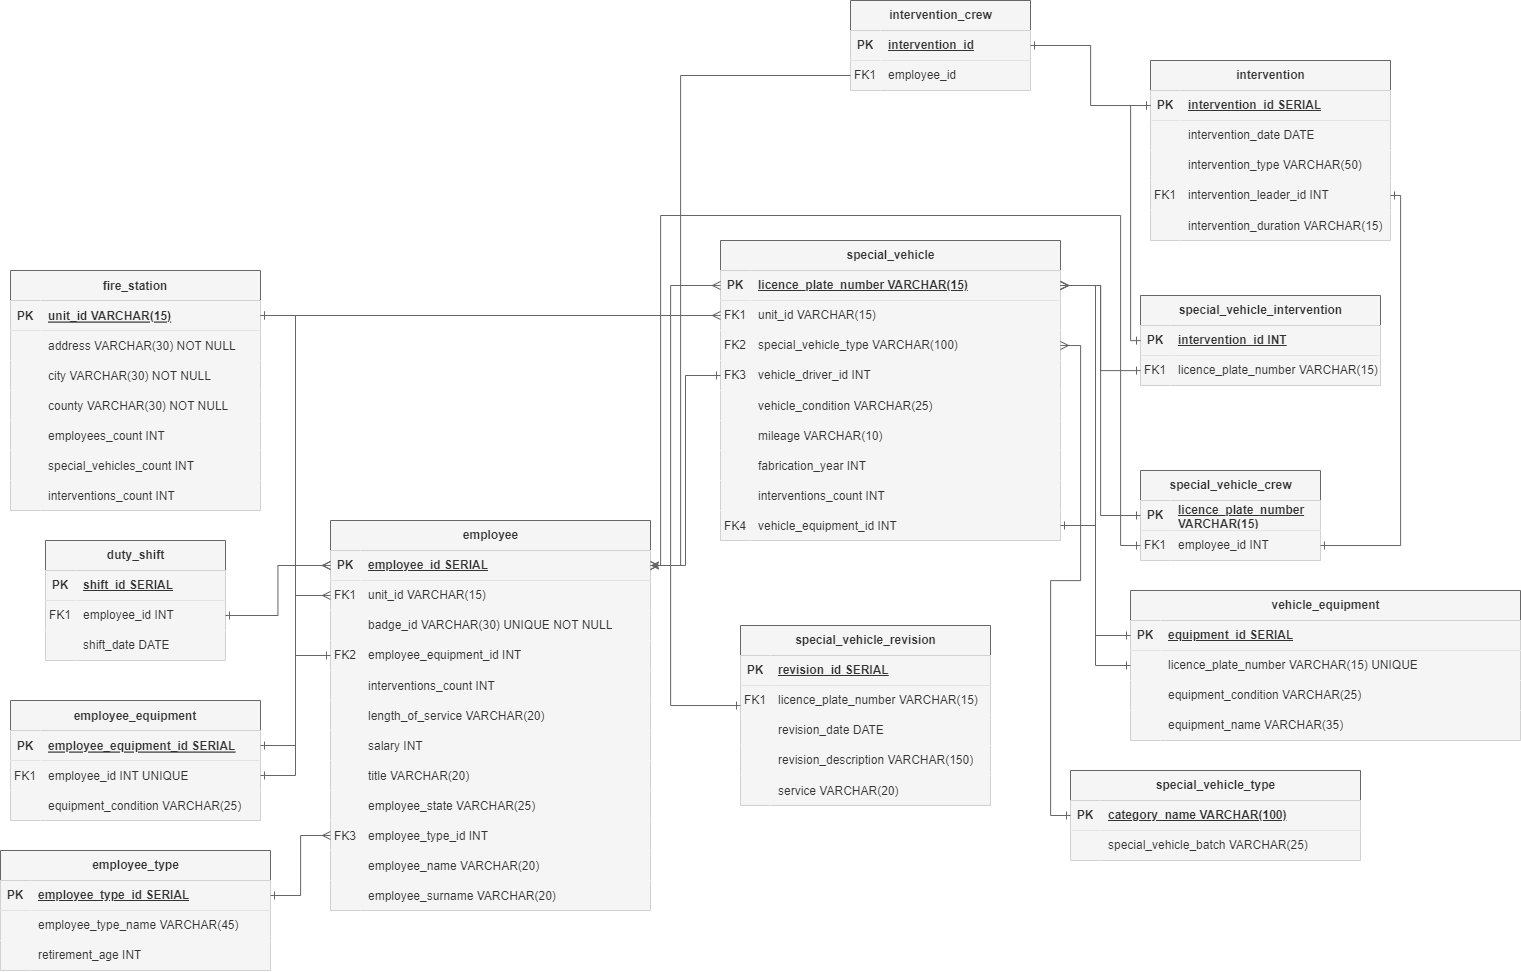
\includegraphics[scale=0.3]{EER.png}

\section{Project contribution}

\begin{itemize}
    \item Drago\c{s}-Alexandru Efrim
    \begin{itemize}
        \item created models, repositories and controllers
        \item created Postman requests
        \item recreated database (in English)
    \end{itemize}
    \item Olivia Drobot
    \begin{itemize}
        \item realised database connection in application.properties
        \item added project tests
        \item research upon information regarding JPA
    \end{itemize}
\end{itemize}

\end{document}
